\subsection{LoS branch: enhanced two ray model}

The LoS prior is not a pure FSPL prior. FSPL is kept because it is the
direct ray normalization term of the coherent two ray model: it gives the
path loss that would be observed if only the direct ray existed. The deployed
LoS branch then adds the fitted ground reflection interference term,
a height dependent bias, and a smoothed radial residual profile. This differs
from the NLoS branch, which uses a longer pixel feature vector and a
regime wise linear calibration.

\subsubsection{Geometry and distances}

Consider a UAV transmitter at height $h_{\mathrm{tx}}$ (metres above the
ground-plane reference) and a receiver at height $h_{\mathrm{rx}}$. For each
map pixel $x$ at 2D horizontal distance $d_{2D}(x)$ from the transmitter, two
propagation distances are defined.

The \emph{direct path} (LoS) distance is:

\begin{equation}
d_{\mathrm{LoS}}(x)
=
\sqrt{d_{2D}(x)^2 + (h_{\mathrm{tx}} - h_{\mathrm{rx}})^2}
\label{eq:d_los}
\end{equation}

This is simply the Euclidean distance between the two antennas in 3D space.
Because \(d_{2D}(x)\ge0\) and the squared height difference
\((h_{\mathrm{tx}}-h_{\mathrm{rx}})^2\) is nonnegative,
\(d_{\mathrm{LoS}}(x) \ge d_{2D}(x)\), with equality only when both antennas
are at the same height.

The \emph{reflected path} (image) distance is:

\begin{equation}
d_{\mathrm{ref}}(x)
=
\sqrt{d_{2D}(x)^2 + (h_{\mathrm{tx}} + h_{\mathrm{rx}})^2}
\label{eq:d_ref}
\end{equation}

This is the distance from the image source (the UAV mirrored below the
ground plane at $-h_{\mathrm{tx}}$) to the receiver. Since $(h_{\mathrm{tx}}
+ h_{\mathrm{rx}}) \ge |h_{\mathrm{tx}} - h_{\mathrm{rx}}|$ for any
nonnegative heights, we always have $d_{\mathrm{ref}}(x) \ge
d_{\mathrm{LoS}}(x)$. In the present UAV to ground setting with
\(h_{\mathrm{tx}}>0\) and \(h_{\mathrm{rx}}>0\), the reflected path is
strictly longer; in the limiting geometric case where one antenna is exactly
on the ground plane, it would be equal rather than longer.

\begin{figure}[H]
\centering
\begin{tikzpicture}[scale=1.0]
\draw[thick] (-0.5,0) -- (6.0,0) node[right] {ground};
\draw[dashed] (-0.5,-3.5) -- (6.0,-3.5) node[right, font=\small] {image source height};

\filldraw[blue] (1.0,3.5) circle(3pt) node[above] {UAV ($h_{\mathrm{tx}}$)};
\filldraw[red]  (5.0,0.5) circle(3pt) node[above right] {Rx ($h_{\mathrm{rx}}$)};
\filldraw[blue!40] (1.0,-3.5) circle(3pt) node[below] {image ($-h_{\mathrm{tx}}$)};

\draw[-{Stealth},thick,blue]  (1.0,3.5) -- (5.0,0.5)
      node[midway, above, sloped, font=\small] {$d_{\mathrm{LoS}}$};

\draw[thick,green!60!black] (1.0,3.5) -- (3.0,0.0);
\draw[thick,green!60!black] (3.0,0.0) -- (5.0,0.5);
\node[above, font=\small, green!60!black] at (2.5,1.6) {reflected};

\draw[dashed,gray] (1.0,-3.5) -- (5.0,0.5)
      node[midway, below, sloped, font=\small, gray] {$d_{\mathrm{ref}}$};

\draw[|<->|] (1.0,-0.1) -- (5.0,-0.1) node[midway, below, font=\small] {$d_{2D}$};
\end{tikzpicture}
\caption[Two ray geometry.]%
{Two ray geometry. Direct path (blue) has length $d_{\mathrm{LoS}}$;
reflected path (green) has the same total length as the image source path
(gray dashed), which is $d_{\mathrm{ref}}$.}
\label{fig:tworay}
\end{figure}

\subsubsection{Free-space path loss baseline}

The free space path loss in dB is defined using the standard formula at
frequency $f_{\mathrm{MHz}}$ (in MHz):

\begin{equation}
\mathrm{FSPL}(x)
=
32.45
+ 20 \log_{10}\!\left(\frac{d_{\mathrm{LoS}}(x)}{1000}\right)
+ 20 \log_{10}(f_{\mathrm{MHz}})
\label{eq:fspl}
\end{equation}

\paragraph{Physical meaning.} FSPL grows quadratically with distance ($\propto
d^2$) and quadratically with frequency. It captures only the geometric
spreading of the wavefront, with no ground interaction, scattering, or
diffraction.

\subsubsection{Enhanced two ray correction}

In the two ray model, the received field is the superposition of the direct
path and a ground reflected path. Let \(\lambda=c/f\) be the wavelength. The
complex sum of the two waves at the receiver is:

\begin{equation}
E_{\mathrm{total}}
\propto
\frac{e^{-j2\pi d_{\mathrm{LoS}}/\lambda}}{d_{\mathrm{LoS}}}
+
\Gamma\,\frac{e^{-j2\pi d_{\mathrm{ref}}/\lambda}}{d_{\mathrm{ref}}}
\label{eq:field_sum}
\end{equation}

where $\Gamma$ is the complex ground reflection coefficient. In the standard
textbook derivation, $\Gamma$ is computed from the Fresnel equations for the
ground material. Here, it is replaced by an \emph{effective} complex
parameter:

\begin{equation}
\Gamma(h_{\mathrm{tx}})
=
\rho(h_{\mathrm{tx}})\,e^{-j\phi(h_{\mathrm{tx}})}
\end{equation}

where $\rho \in [0, 1.5]$ is the effective amplitude used during the
calibration search and $\phi \in [-\pi,\pi]$ is the effective phase offset.
The search range is only a robustness allowance for a fitted CKM parameter, not
a claim that a passive ground reflection coefficient exceeds unity; the
deployed smoothed values reported later remain below one.
Both parameters depend on the UAV height bin.

The two ray path loss correction term in dB is:

\begin{equation}
C_{\mathrm{2ray}}(x)
=
-20 \log_{10}
\left|
1 + \rho(h_{\mathrm{tx}})
\frac{d_{\mathrm{LoS}}(x)}{d_{\mathrm{ref}}(x)}
e^{-j\left(2\pi\frac{d_{\mathrm{ref}}(x)-d_{\mathrm{LoS}}(x)}{\lambda}+\phi(h_{\mathrm{tx}})\right)}
\right|
\label{eq:c2ray}
\end{equation}

\paragraph{Term by term interpretation.}
\begin{itemize}
\item $\rho(h_{\mathrm{tx}})$: amplitude of the ground reflection. A value of
      $\rho = 0$ recovers pure FSPL. The fitted values are $\rho \approx
      0.46$ to $0.56$ for heights 10 to 100 m, consistent with a moderate
      ground reflection coefficient.
\item $d_{\mathrm{LoS}}(x)/d_{\mathrm{ref}}(x)$: path amplitude ratio. This
      is always $\le 1$ since the reflected path is longer; it corrects for
      the $1/d$ amplitude decay of the reflected ray relative to the direct
      ray.
\item \(2\pi(d_{\mathrm{ref}}(x)-d_{\mathrm{LoS}}(x))/\lambda\): the phase
      difference accumulated due to the extra path length of the reflected
      wave.
\item $\phi(h_{\mathrm{tx}})$: an additional phase offset capturing phase
      shifts upon reflection (e.g., phase shift at the boundary). The fitted
      values are $\phi \approx 0$ for all height bins, meaning the fitted
      extra phase offset is near zero under this sign convention.
\item $-20\log_{10}|\cdot|$: the total field amplitude at the receiver,
      normalized to the direct path field. When the two waves add in phase, the
      field amplitude is $> 1$, giving a \emph{negative} correction (the signal
      is \emph{stronger} than FSPL alone); when they cancel, the correction is
      \emph{positive} (fading loss).
\end{itemize}

This spatial interference pattern creates the characteristic ring like
behavior in the LoS path loss maps: concentric rings of constructive and
destructive interference around the transmitter.

\subsubsection{Comparison with literature two ray models}

The field sum in \eqref{eq:c2ray} is the standard \emph{exact} coherent
two ray equation from the literature: a direct ray plus one ground reflected
ray summed before conversion to dB. The practical adaptation in this thesis
is not an extra term inside the two ray equation, but the way the reflection
coefficient is parameterized and calibrated. We refer to this fitted variant
as the \emph{enhanced two ray} model throughout this work: the underlying
equation is the textbook coherent two ray model, but the effective reflection
coefficient is enhanced beyond the Fresnel range and allowed to take
amplitudes up to $\rho \le 1.5$ in order to absorb constructive multipath
effects from the surrounding urban scene that a single Fresnel coefficient
could not represent. The coefficients are fitted
independently in 5~m UAV height bins and then linearly interpolated across
neighboring bins at inference time.

\paragraph{Physical vs.\ effective parameters.}
Classical two ray models usually derive \(\Gamma\) from a smooth ground
material and a grazing angle \cite{rappaport,goldsmith}. The thesis does not
assume one flat dielectric plane. It keeps the coherent direct plus reflected
field sum, but replaces the material coefficient with a height dependent
effective coefficient \(\Gamma(h_{\mathrm{tx}})=\rho e^{-j\phi}\), fitted from
training-city CKM LoS pixels in \SI{5}{m} UAV height bins and linearly
interpolated at inference. Thus \(\rho\) is an effective reflected field
amplitude and \(\phi\) is the extra fitted phase offset of the simplified one
reflection geometry.

\paragraph{Search range vs.\ fitted values.}
The calibration grid search (Sec.~\ref{sec:los_calibration}) allows
$\rho \in [0, 1.5]$ for robustness. However, the smoothed deployed values
reported in Table~\ref{tab:los_params} and the stored calibration remain below
unity, so the deployed model does not rely on an over unity reflected ray. In
practice, the main difference from a purely physical textbook instantiation is
therefore the fitted height binned effective coefficient, not an additional
propagation term.

\paragraph{Extra calibrated terms outside the two ray model.}
The quantities $b(h_{\mathrm{tx}})$ and $r(d_{2D}, h_{\mathrm{tx}})$ in
\eqref{eq:pl_los} are not part of the literature two ray formula itself.
They are post fit calibration terms added on top of the standard two ray
prediction to absorb residual systematic errors.

\subsubsection{Calibrated LoS prior}

The full calibrated LoS prior is:

\begin{equation}
\mathrm{PL}_{\mathrm{LoS}}(x)
=
\mathrm{FSPL}(x)
+ C_{\mathrm{2ray}}(x)
+ b(h_{\mathrm{tx}})
+ r(d_{2D}(x), h_{\mathrm{tx}})
\label{eq:pl_los}
\end{equation}

where:
\begin{itemize}
\item $b(h_{\mathrm{tx}})$ is a height dependent bias (dB): a constant
      correction that shifts the overall two ray prediction for a given UAV
      height.
\item $r(d_{2D}(x), h_{\mathrm{tx}})$ is a radial residual correction: a
      smooth function of horizontal distance (and height bin) that captures
      systematic over-/under-prediction of the two ray model as a function of
      range. It is obtained by smoothing the empirical mean residual in each
      distance bin after the two ray fit.
\end{itemize}

The four terms in \eqref{eq:pl_los} are applied sequentially:
FSPL gives the geometric baseline; the two ray correction adds the
interference pattern; the bias corrects for a systematic global offset per
height; and the radial term corrects for range dependent systematic errors.
The implementation then clips the frozen LoS prior to the \([20,180]\) dB
range used by the final model. For the CKM dataset used here, valid calibrated
LoS values are not expected to fall outside this interval, so this clipping is
a defensive range consistency guard rather than a correction that should
materially change the prior.

For compact notation, the LoS branch can be summarized by the following
deterministic diagnostic vector:

{\small
\begin{equation}
\mathbf{q}_{\mathrm{LoS}}(x)
=
\begin{bmatrix}
\mathrm{FSPL}(x)\\
d_{\mathrm{LoS}}(x)/d_{\mathrm{ref}}(x)\\
2\pi(d_{\mathrm{ref}}(x)-d_{\mathrm{LoS}}(x))/\lambda\\
\rho(h_{\mathrm{tx}})\\
\phi(h_{\mathrm{tx}})\\
C_{\mathrm{2ray}}(x)\\
b(h_{\mathrm{tx}})\\
r(d_{2D}(x),h_{\mathrm{tx}})
\end{bmatrix}.
\label{eq:pl_los_diagnostic_vector}
\end{equation}
}

This diagnostic vector is not multiplied by a learned coefficient vector at inference
time. Instead, it exposes the calibrated quantities used by the nonlinear
two ray expression
\(\mathrm{PL}_{\mathrm{LoS}}(x)
=g_{\mathrm{LoS}}(\mathbf{q}_{\mathrm{LoS}}(x))
=\mathrm{FSPL}(x)+C_{\mathrm{2ray}}(x)+b(h_{\mathrm{tx}})
+r(d_{2D}(x),h_{\mathrm{tx}})\).
The entries are computed as follows:

\begin{itemize}
\item \(\mathrm{FSPL}(x)\) is computed from the 3D direct distance
      \(d_{\mathrm{LoS}}(x)\) and the carrier frequency. It is the
      direct ray path loss, so it sets the absolute distance and frequency
      scale before any reflected path correction is added.
\item \(d_{\mathrm{LoS}}(x)/d_{\mathrm{ref}}(x)\) is computed from the
      direct path length and the image source reflected path length. Since the
      reflected path is longer, this ratio is normally below one and gives the
      relative amplitude of the reflected field after \(1/d\) propagation loss.
\item \(2\pi(d_{\mathrm{ref}}(x)-d_{\mathrm{LoS}}(x))/\lambda\) is the
      geometric phase advance of the reflected ray. This is the term that makes
      the correction oscillatory in space: small changes in extra path length
      can move the direct and reflected fields from constructive to destructive
      interference.
\item \(\rho(h_{\mathrm{tx}})\) is the effective reflection amplitude used in
      the coherent field sum. During calibration, each 5 m UAV height bin is
      fitted by grid search over \(\rho\in[0,1.5]\) and the phase grid; for
      each candidate pair, the best constant bias is removed and the pair with
      lowest LoS RMSE is selected. The stored \(\rho\) curve is then smoothed
      across neighboring height bins and, at inference time, linearly
      interpolated to the actual \(h_{\mathrm{tx}}\). Thus \(\rho\) is not a
      Fresnel coefficient assumed from a ground material, but a CKM-calibrated
      effective reflected field amplitude.
\item \(\phi(h_{\mathrm{tx}})\) is fitted in the same height binned grid
      search, using a uniform grid over \([-\pi,\pi)\). It absorbs the
      effective phase shift of the reflection and any systematic phase offset
      caused by the simplified one reflection geometry. As with \(\rho\), the
      stored phase curve is smoothed across height bins and linearly
      interpolated during prediction.
\item \(C_{\mathrm{2ray}}(x)\) is then computed by substituting
      \(d_{\mathrm{LoS}}/d_{\mathrm{ref}}\), the geometric phase,
      \(\rho(h_{\mathrm{tx}})\), and \(\phi(h_{\mathrm{tx}})\) into
      \eqref{eq:c2ray}. This is the actual coherent direct plus reflected
      correction in dB. A negative value means constructive gain relative to
      FSPL; a positive value means a fading loss.
\item \(b(h_{\mathrm{tx}})\) is the constant dB offset fitted together with
      \(\rho\) and \(\phi\) for each height bin. For a fixed candidate
      \((\rho,\phi)\), the calibration computes the mean residual
      \(y-(\mathrm{FSPL}+C_{\mathrm{2ray}})\) over the sampled LoS pixels in
      that height bin and uses it as the optimal bias for that candidate. The
      final stored \(b\) is smoothed over height and linearly interpolated at
      inference time. Its role is to remove the remaining height dependent
      offset after the interference pattern has been fitted.
\item \(r(d_{2D}(x),h_{\mathrm{tx}})\) is fitted after the smoothed two ray
      model is fixed. The residual target-minus-prediction is accumulated in
      integer radial bins around the transmitter, separately for each
      5 m height bin; empty bins fall back to a global radial profile, the
      profile is smoothed, and the applied correction is clipped to
      \(\pm2.5\) dB. This term removes range dependent structure that remains
      after the coherent two ray model and the height bias.
\end{itemize}

\begin{table}[H]
\centering
\footnotesize
\setlength{\tabcolsep}{4pt}
\renewcommand{\arraystretch}{1.08}
\begin{tabularx}{\textwidth}{p{3.2cm} X X}
\toprule
\textbf{Stored / computed term} & \textbf{Mathematical role} & \textbf{Interpretation} \\
\midrule
\(\mathrm{FSPL}(d_{\mathrm{LoS}},f)\) & Direct ray baseline. & Gives the geometric free space loss before any reflected path is added. It is a component of the two ray prior, not the final LoS model by itself. \\
\(\rho(h_{\mathrm{tx}})\) & Height interpolated reflected ray amplitude. & Controls how strongly the ground reflected wave contributes relative to the direct wave. \\
\(\phi(h_{\mathrm{tx}})\) & Height interpolated phase offset. & Captures the effective reflection phase after fitting to CKM instead of assuming a fixed Fresnel coefficient. \\
\(C_{\mathrm{2ray}}(x)\) & Coherent interference correction. & Converts the complex direct plus reflected field sum into an oscillatory dB correction around FSPL. \\
\(b(h_{\mathrm{tx}})\) & Height interpolated bias. & Removes a remaining per height offset after the coherent two ray fit. \\
\(r(d_{2D},h_{\mathrm{tx}})\) & Smoothed radial residual profile, clipped to \(\pm2.5\) dB. & Corrects systematic distance dependent residuals not captured by the two ray equation. \\
\(\mathrm{clip}_{[20,180]}\) & Output guard. & Keeps the frozen prior inside the physical path loss range used by the final model. \\
\bottomrule
\end{tabularx}
\caption{Term by term inventory of the LoS prior used by
the final model. Unlike the NLoS branch, this is not a long pixel feature
regression vector; it is a height-interpolated two ray calibration plus a
radial residual table.}
\label{tab:pl_los_term_inventory}
\end{table}

\subsection{Calibration of the LoS two ray model}
\label{sec:los_calibration}

\subsubsection{Data preparation}

All training samples are used. For each sample, valid LoS pixels are selected
as those satisfying:
\begin{enumerate}
\item topology label = 0 (ground pixel),
\item $m_{\mathrm{LoS}}(x) > 0$ (marked as LoS),
\item the measured path loss is finite and $\ge 20$ dB.
\end{enumerate}
If a sample has more than 2\,500 valid LoS pixels, a random subsample of
2\,500 pixels is drawn (with a fixed seed). Samples are then grouped by UAV
height into height bins of 5 m width:

\begin{equation}
h_{\mathrm{bin}} = 5 \cdot \operatorname{round}\!\left(\frac{h_{\mathrm{tx}}}{5}\right)
\end{equation}

Each bin is further subsampled to a maximum of 8\,000 pixels total.

\subsubsection{Grid search for $(\rho, \phi)$}

For each height bin, $(\rho, \phi)$ are found by grid search:

\begin{align}
\phi_{\mathrm{grid}} &= \left\{-\pi + \frac{2\pi q}{N_\phi} : q = 0, 1, \ldots, N_\phi - 1\right\},
\quad N_\phi = 48 \label{eq:phi_grid}\\
\rho_{\mathrm{grid}} &= \{0.00,\, 0.05,\, 0.10,\, \ldots,\, 1.50\}
\label{eq:rho_grid}
\end{align}

For each pair $(\hat\rho, \hat\phi) \in \rho_{\mathrm{grid}} \times
\phi_{\mathrm{grid}}$, and for each pixel $x_i$ in the height bin, define
the two ray prediction without bias:

\begin{equation}
\hat p_i(\hat\rho, \hat\phi)
=
\mathrm{FSPL}(x_i)
- 20\log_{10}
\left|
1 + \hat\rho\,\frac{d_{\mathrm{LoS}}(x_i)}{d_{\mathrm{ref}}(x_i)}
e^{-j\left(2\pi\frac{d_{\mathrm{ref}}(x_i)-d_{\mathrm{LoS}}(x_i)}{\lambda}+\hat\phi\right)}
\right|
\end{equation}

The optimal bias for each $(\hat\rho, \hat\phi)$ pair is solved analytically
as the empirical mean of residuals:

\begin{equation}
\hat b(\hat\rho, \hat\phi)
=
\frac{1}{N}\sum_{i=1}^{N}
\left(y_i - \hat p_i(\hat\rho, \hat\phi)\right)
\end{equation}

where $y_i$ is the measured path loss at pixel $x_i$ and $N$ is the number
of pixels in the bin. The biased prediction is $\hat p_i + \hat b$, and the
RMSE for the pair is:

\begin{equation}
\mathrm{RMSE}(\hat\rho, \hat\phi)
=
\sqrt{\frac{1}{N}\sum_{i=1}^{N}
\left(y_i - \hat p_i(\hat\rho,\hat\phi) - \hat b(\hat\rho,\hat\phi)\right)^2}
\label{eq:rmse_grid}
\end{equation}

The best pair is:

\begin{equation}
(\rho^*, \phi^*)
= \arg\min_{(\hat\rho, \hat\phi)}
\mathrm{RMSE}(\hat\rho, \hat\phi)
\end{equation}

\subsubsection{Post fit Gaussian smoothing across height bins}

After fitting all bins independently, a Gaussian-weighted smooth is applied
to stabilize sparse high altitude bins. Let $\{h_k\}$ be the fitted height
bin centers, $\{(\rho_k^*, \phi_k^*, b_k^*)\}$ the per bin fitted values,
and $\{N_k\}$ the pixel counts used in fitting. The implementation weights
each bin by $\sqrt{N_k}$ rather than by $N_k$ itself, so very populated bins
stabilize the curve without completely dominating neighboring sparse bins.
The smoothed values are:

\begin{equation}
\tilde\rho(h)
=
\frac{\sum_k w_k(h)\sqrt{N_k}\,\rho_k^*}{\sum_k w_k(h)\sqrt{N_k}},
\qquad
w_k(h) = \exp\!\left(-\frac{(h - h_k)^2}{2\sigma_h^2}\right),
\quad \sigma_h = 10\;\mathrm{m}
\label{eq:gauss_smooth}
\end{equation}

and similarly for $\phi$ and $b$. The implementation also stores a
suspicious-bin mask for bins where both $\rho_k^*$ and $b_k^*$ differ
noticeably from the smoothed global trend, typically high altitude bins with
few samples. That mask is diagnostic metadata: the runtime calibration arrays
used by the final residual model are the smoothed $\rho$, $\phi$, and $b$ curves themselves, not
a mixture of raw values for ordinary bins and smoothed values only for flagged
ones.
At inference time the UAV height is not forced to be exactly one of the fitted
5 m bin centers. The implementation linearly interpolates $\rho(h_{\mathrm{tx}})$,
$\phi(h_{\mathrm{tx}})$, $b(h_{\mathrm{tx}})$, and the radial residual profile
between the two nearest height bins, and clamps to the nearest endpoint outside
the fitted range. This keeps the prior continuous with respect to UAV height
instead of introducing discrete jumps every 5 m.

\subsubsection{Radial residual correction}

After fitting the two ray model, a residual correction is computed separately
per height bin and integer radius:

\begin{equation}
r(r_{\mathrm{px}},h_{\mathrm{tx}})
=
\mathrm{clip}\!\left(
\mathrm{GaussSmooth}_{\sigma_r}\left(
\mathbb{E}_{h\text{-bin},\,r_{\mathrm{px}}}
\left[
\mathrm{clip}\!\left(y-\hat y_{\mathrm{2ray}},-2.5,+2.5\right)
\right]
\right)
\!, -2.5,+2.5
\right)
\end{equation}

where $r_{\mathrm{px}}$ is the rounded 2D pixel radius from the transmitter,
$\sigma_r = 1.5$ pixels is the Gaussian smoothing radius, and the $\pm2.5$ dB
clip is applied both to individual residual samples during accumulation and
to the interpolated profile used at inference. Radius bins with no samples in
a height bin fall back to the global radial profile before smoothing. At
inference, the profile is linearly interpolated across the stored height bins,
then indexed by the pixel-radius map and added to the coherent two ray
prediction.

\subsubsection{Smoothed deployed parameter values}

Table~\ref{tab:los_params} shows representative LoS two ray parameters after
the post fit Gaussian smoothing across height bins. These are the deployed
calibration values used by the prior at inference time, not the unsmoothed
per bin grid-search optima.

\begin{table}[H]
\centering
\caption{Representative smoothed deployed LoS two ray parameters by height bin.}
\label{tab:los_params}
\small
\begin{tabular}{rrrr}
\toprule
$h_{\mathrm{tx}}$ (m) & $\tilde{\rho}$ & $\tilde{\phi}$ (rad) & $\tilde{b}$ (dB)\\
\midrule
10  & 0.5605 & 0.000 & $-$0.037 \\
20  & 0.5242 & 0.000 & $-$0.042 \\
30  & 0.4950 & 0.000 & $-$0.042 \\
50  & 0.4632 & 0.000 & $-$0.047 \\
80  & 0.4958 & 0.000 & $-$0.013 \\
100 & 0.4926 & 0.000 & $-$0.011 \\
140 & 0.5308 & 0.000 & $-$0.028 \\
460 & 0.8966 & $-$0.030 & $+$1.432 \\
\bottomrule
\end{tabular}
\end{table}

The dominant deployed pattern is $\tilde{\rho} \approx 0.46$ to $0.56$ with
$\tilde{\phi} \approx 0$ for heights 10 to 100 m, meaning a moderate-amplitude
ground reflection with a near zero fitted extra phase offset. Biases are
near zero ($< 0.05$ dB) for these bins. At very high altitudes, the smoothed
deployed $\tilde{\rho}$ and bias increase because training data is sparser;
those bins are stabilized by Gaussian smoothing before deployment.

\begin{figure}[H]
\centering
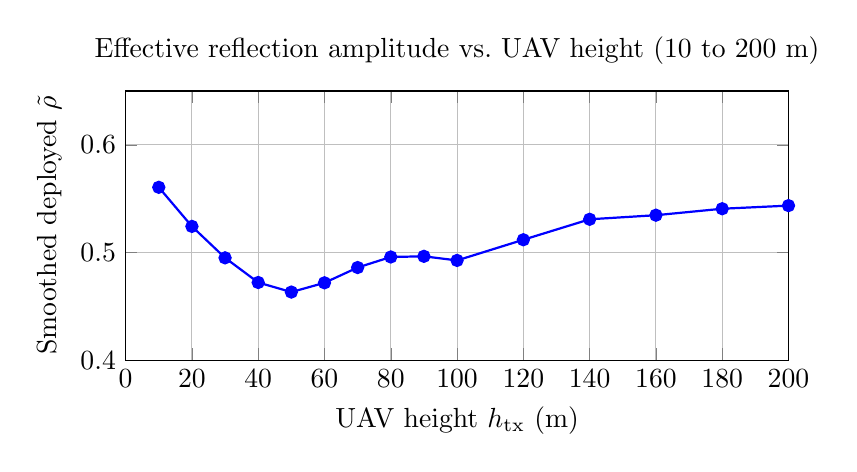
\begin{tikzpicture}
\begin{axis}[
  width=10cm, height=5cm,
  xlabel={UAV height $h_{\mathrm{tx}}$ (m)},
  ylabel={Smoothed deployed $\tilde{\rho}$},
  xmin=0, xmax=200,
  ymin=0.4, ymax=0.65,
  grid=major,
  title={Effective reflection amplitude vs.\ UAV height (10 to 200 m)}
]
\addplot[mark=*, thick, blue] coordinates {
  (10,0.5605)(20,0.5242)(30,0.4950)(40,0.4721)
  (50,0.4632)(60,0.4718)(70,0.4860)(80,0.4958)
  (90,0.4964)(100,0.4926)(120,0.5118)(140,0.5308)
  (160,0.5346)(180,0.5406)(200,0.5435)
};
\end{axis}
\end{tikzpicture}
\caption[Effective ground reflection amplitude as a function of UAV height.]
{Effective ground reflection amplitude $\tilde{\rho}$ as a function of UAV
height after post fit smoothing across 5 m height bins. Values are stable in
the range $0.46$ to $0.56$ for 10 to 200 m, then rise at the sparsely sampled
very-high altitude bins used by the calibration.}
\label{fig:rho_vs_h}
\end{figure}

\begin{figure}[H]
\centering
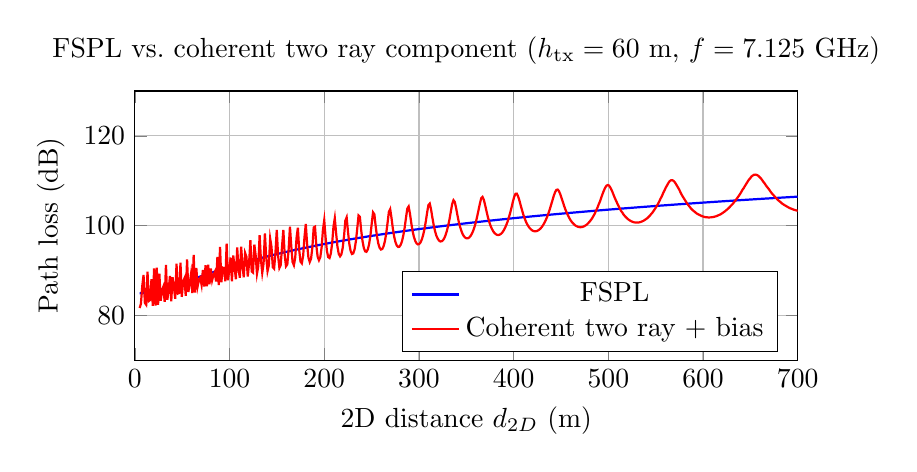
\begin{tikzpicture}
\begin{axis}[
  width=10cm, height=5cm,
  xlabel={2D distance $d_{2D}$ (m)},
  ylabel={Path loss (dB)},
  xmin=0, xmax=700,
  ymin=70, ymax=130,
  xtick={0,100,200,300,400,500,600,700},
  grid=major,
  legend pos=south east,
  title={FSPL vs.\ coherent two ray component ($h_{\mathrm{tx}} = 60$ m, $f = 7.125$ GHz)}
]
\addplot[thick, blue, domain=5:700, samples=500]
  {32.45 + 20*ln(sqrt(x^2+3422.25)/1000)/ln(10) + 20*ln(7125)/ln(10)};
\addlegendentry{FSPL}
\addplot[thick, red, domain=5:700, samples=500]
  {32.45 + 20*ln(sqrt(x^2+3422.25)/1000)/ln(10) + 20*ln(7125)/ln(10)
   - 20*ln(sqrt((1 + 0.4718 * sqrt(x^2+3422.25)/sqrt(x^2+3782.25) *
   cos(deg(2*3.14159*(sqrt(x^2+3782.25)-sqrt(x^2+3422.25))*7125e6/3e8)))^2
   + (0.4718 * sqrt(x^2+3422.25)/sqrt(x^2+3782.25) *
   sin(deg(2*3.14159*(sqrt(x^2+3782.25)-sqrt(x^2+3422.25))*7125e6/3e8)))^2))/ln(10)
   - 0.044};
\addlegendentry{Coherent two ray + bias}
\end{axis}
\end{tikzpicture}
\caption[FSPL versus coherent two ray component.]%
{Schematic comparison of FSPL and the calibrated coherent two ray component for
a 60 m UAV at 7.125 GHz ($h_{\mathrm{rx}} = 1.5$ m), zoomed to the
\SI{700}{m} near field that contains the full \(513\times513\) map diagonal.
The plotted red curve uses the code loaded 60 m calibration values before
adding the radial residual profile, so it shows the constructive/destructive
interference term rather than the full final LoS prior.}
\label{fig:tworay_pl}
\end{figure}

\subsection{NLoS branch}
\label{sec:nlos_branch}

The NLoS path loss branch used in the final model is not a pure literature
formula. It is a hybrid engineering model built in five stages.

\subsubsection{Stage 1: raw NLoS propagation prior}

Two coarse physical estimates are combined.

\paragraph{COST-231 term.}
The COST-231 / Hata extension for urban macro cells gives the empirical
large scale path loss expression used below \cite{cost231}. It is included
because it is one of the standard references for urban NLoS macrocell loss,
even though the CKM scenario is outside its original frequency and base station
height range. None of the COST-231 coefficients is therefore treated as a
physically transferred absolute predictor at \SI{7.125}{GHz}; the equation is
only a log distance and height sensitive basis that the train only NLoS
calibration can bend:

\begin{equation}
\begin{aligned}
\mathrm{PL}_{\mathrm{COST231}}(x)
={}&
46.3 + 33.9 \log_{10}(f_{\mathrm{MHz}})
- 13.82 \log_{10}(h_{\mathrm{tx}})
- a(h_{\mathrm{rx}})\\
&+
\left(44.9 - 6.55 \log_{10}(h_{\mathrm{tx}})\right)
\log_{10}(d_{\mathrm{km}})
+ 3
\end{aligned}
\label{eq:cost231}
\end{equation}

where $d_{\mathrm{km}} = \max(d_{2D}(x)/1000, 0.001)$ and the implemented
mobile antenna correction is the COST-231 small/medium city correction:

\begin{equation}
a(h_{\mathrm{rx}})
=
\left(1.1\log_{10}(f_{\mathrm{MHz}})-0.7\right)h_{\mathrm{rx}}
-
\left(1.56\log_{10}(f_{\mathrm{MHz}})-0.8\right)
\label{eq:cost231_a}
\end{equation}

\eqref{eq:cost231} should therefore be read as a calibrated
\emph{feature basis}, not as a trusted absolute predictor or as a claim that
COST-231 itself transfers to this \SI{7.125}{GHz} UAV geometry. COST-231
contributes the expected log distance growth, transmitter height dependence and
receiver height correction of an urban empirical model. The subsequent
train only calibration stage is what adapts that shape to the ray tracing
setting used here.

\paragraph{Interpretation of \eqref{eq:cost231}.}
\begin{itemize}
\item $46.3 + 33.9\log_{10}(f_{\mathrm{MHz}})$: frequency dependent offset.
      The coefficient $33.9$ (compare to $20$ for FSPL) reflects stronger
      frequency dependence in urban scattering.
\item $-13.82\log_{10}(h_{\mathrm{tx}})$: as the base station / UAV gets
      higher, path loss decreases (better clearance above rooftops). The
      $-13.82$ coefficient is a fitted constant from the Hata empirical
      dataset.
\item $-a(h_{\mathrm{rx}})$: accounts for the receiver height using the
      implemented small/medium city Hata correction. For typical pedestrian
      heights ($h_{\mathrm{rx}} \approx 1.5$ m), this is a small offset
      relative to the distance and height terms.
\item $(44.9 - 6.55\log_{10}(h_{\mathrm{tx}}))\log_{10}(d_{\mathrm{km}})$:
      distance dependent term. The effective path loss exponent is
      $(44.9 - 6.55\log_{10}(h_{\mathrm{tx}}))/10$, which decreases as the
      UAV climbs (effectively reducing NLoS scattering losses at longer
      distances from higher altitudes).
\item $+3$: the COST-231 metropolitan correction constant (dB), corresponding
      to the dense-urban correction in the original model \cite{cost231}.
      In this thesis it is retained only as an implementation basis constant,
      together with the small/medium city receiver height correction in
      \eqref{eq:cost231_a}. This deliberate mixture is not a canonical
      COST-231 deployment recipe; it is one empirical axis later refitted by
      the regime wise calibration.
\end{itemize}

\paragraph{Elevation-aware UAV envelope.}
The A2G NLoS envelope is used as a conservative elevation dependent shape term
for urban air to ground path loss. UAV channel models motivate elevation angle
as an important modelling axis because obstruction and shadowing statistics vary
with elevation \cite{khawaja_survey,tr38901}. The particular constants below,
however, are not used as a transferred monotonic law. With the positive
exponential term, the raw envelope can be larger near overhead; it is therefore
only one conservative basis branch that is later combined with COST-231 through
a maximum and corrected by the train only regime wise NLoS calibration.

\begin{equation}
\mathrm{PL}_{\mathrm{A2G,NLoS}}(x)
=
\lambda_0(h_{\mathrm{tx}}, f)
+ \beta_{\mathrm{NLoS}}
+ A_{\mathrm{NLoS}}
\exp\!\left(-\frac{90-\theta^\circ(x)}{\tau_{\mathrm{NLoS}}}\right)
\label{eq:a2g_nlos}
\end{equation}

where:
\begin{align}
\lambda_0(h_{\mathrm{tx}}, f)
&= 20\log_{10}\!\left(\frac{4\pi h_{\mathrm{tx}} f}{c}\right)
\label{eq:lambda0}
\end{align}

The fixed A2G-envelope constants used by the implementation are:
$\beta_{\mathrm{NLoS}} = -16.16$ dB,
$A_{\mathrm{NLoS}} = 12.0436$,
$\tau_{\mathrm{NLoS}} = 7.52$ deg.
These A2G constants are implementation constants in the path-loss prior code
rather than entries in the calibration JSON files; the JSON artifacts store the
fitted LoS two ray curves and the regime wise NLoS calibration coefficients.

\paragraph{Interpretation of \eqref{eq:a2g_nlos}.}
\begin{itemize}
\item $\lambda_0$: the free space reference level used inside the raw A2G NLoS
      envelope before the empirical NLoS offset and elevation angle modulation
      are applied~\cite{khawaja_survey,wocc2021}. The CKM dataset uses
      $f = 7.125$ GHz (FR3 6G frequency band); for
      $h_{\mathrm{tx}} = 50$ m at that frequency, $\lambda_0 \approx 83.5$ dB.
\item $\beta_{\mathrm{NLoS}} = -16.16$ dB: a fixed baseline offset relative
      to $\lambda_0$ in the raw A2G envelope.
\item $A_{\mathrm{NLoS}}\exp(-\ldots)$: an exponential modulation with
      $(90 - \theta^\circ)$. When the elevation angle $\theta^\circ$ is high
      (UAV nearly overhead, $\theta^\circ \to 90^\circ$), the exponent
      vanishes and the term goes to \(A_{\mathrm{NLoS}}\). When
      \(\theta^\circ\) is low (grazing incidence), the exponent is large and
      the term approaches zero. With the current positive
      \(A_{\mathrm{NLoS}}=12.0436\), this raw envelope therefore adds a larger
      A2G offset at high elevation. The later
      \(\max(\mathrm{COST231},\mathrm{A2G})\) switch and the regime wise NLoS
      calibration decide whether that branch is active in the final raw prior;
      it should be read as a fitted conservative envelope, not as a standalone
      monotonic law saying all overhead NLoS links have lower loss.
\item $\tau_{\mathrm{NLoS}} = 7.52^\circ$: the characteristic angular scale.
      A low value means the transition from grazing to overhead happens
      sharply within a small elevation range.
\end{itemize}

The raw NLoS prior is then the conservative (higher) of the two estimates:

\begin{equation}
\mathrm{PL}_{\mathrm{NLoS,raw}}(x)
=
\max\left(
\mathrm{PL}_{\mathrm{COST231}}(x),
\mathrm{PL}_{\mathrm{A2G,NLoS}}(x)
\right)
\label{eq:nlos_raw}
\end{equation}

The maximum in \eqref{eq:nlos_raw} is deliberately pessimistic. If the
empirical COST-231 curve predicts stronger attenuation than the A2G envelope,
the model keeps the urban macro value; if the elevation aware envelope predicts
stronger attenuation, the model keeps the A2G value. This prevents the raw
prior from becoming unrealistically optimistic in NLoS streets where neither
source model is fully valid on its own.

\subsubsection{Stage 2: raw formula map for NLoS calibration}

The NLoS construction above defines only the obstructed branch. The
calibration feature \(\mathrm{PL}^{(0)}(x)\) is the raw formula map used as an
anchor for the NLoS regressor. It is not the final channel attenuation prior.
The implementation forms it by hard switching between an auxiliary LoS formula
helper and the conservative raw NLoS branch:

\begin{equation}
\mathrm{PL}^{(0)}(x)
=
m_{\mathrm{LoS}}(x)\,\mathrm{PL}_{\mathrm{LoS,aux}}(x)
+
\left(1-m_{\mathrm{LoS}}(x)\right)\mathrm{PL}_{\mathrm{NLoS,raw}}(x)
\label{eq:pl0}
\end{equation}

The auxiliary term \(\mathrm{PL}_{\mathrm{LoS,aux}}\) is only a legacy formula
helper used to keep \(\mathrm{PL}^{(0)}\) defined over the whole map. In the
final frozen path, LoS output pixels come directly from the separate enhanced
two ray prior \(\mathrm{PL}_{\mathrm{LoS}}\) of \eqref{eq:pl_los}; the raw
formula map \(\mathrm{PL}^{(0)}\) in \eqref{eq:pl0} is used only as one input
feature for the calibrated NLoS branch.
The LoS/NLoS mask used here is the explicit CKM mask provided with the
dataset and treated as an available side channel. A deployment version would
need to obtain an equivalent visibility mask from deterministic geometry or
another inexpensive pre-processing step; replacing the supplied mask is not
evaluated in this thesis.

\subsubsection{Stage 3: map derived morphology features}

The raw hybrid prior $\mathrm{PL}^{(0)}(x)$ defined in \eqref{eq:pl0} is
the scalar formula input to the calibrated NLoS path loss branch. It combines the
legacy FSPL/two ray LoS path, the A2G envelopes and COST-231, but it still
knows nothing about the detailed local morphology around each receiver. The
feature vector $\mathbf{x}_{\mathrm{PL,NLoS}}(x)$ defined below is \emph{not} a competing
path loss model and \emph{not} an alternative two ray formulation. It is the
per pixel input row of a calibrated linear regressor whose role is to take
the raw formula prediction and absorb its residual using context that the
formula cannot see (urban morphology, NLoS visibility, shadowing and
elevation geometry). Concretely, $\mathrm{PL}^{(0)}(x)$ is fed in as the
dominant feature, plus a quadratic of itself so that the linear fit can bend
the prior, and every other entry adds a quantity that is invisible to the raw
formula.

From $\mathrm{PL}^{(0)}(x)$ and the map topology, a 15-element feature
vector is computed:

The choice of these features is deliberately close to classical urban
propagation modelling, but adapted to the dense CKM setting. The broad
motivation is the COST 231 Walfisch Ikegami model: urban NLoS loss depends on
the surrounding built form, not only on distance and frequency \cite{cost231}.
The Walfisch Bertoni part represents rows of buildings as repeated diffraction
screens \cite{walfisch1988}. The Ikegami street level part motivates
descriptors such as mean building height, street width, street orientation with
respect to the link, and mobile height \cite{ikegami1984}. In this thesis those
planning variables are replaced by quantities measured directly around each
receiver in the 513 by 513 topology map: windowed building density, local mean
building height, and local NLoS support. The elevation and LoS/NLoS split
follow the same physical intuition as A2G models, where shadowing and blockage
statistics vary strongly with elevation angle and environment type
\cite{alhourani2014,khawaja_survey}. The closest modern machine learning
analogue is Juang's path profile work, which uses building profile statistics
in a linear surrogate for urban path loss \cite{juang2021pathprofile}. The
calibrated NLoS branch keeps that explanatory spirit, but fits the coefficients
on training city pixels only and applies the resulting calibration as a frozen
prior rather than as a universal propagation law.

\begin{equation}
\textbf{x}_{\mathrm{PL,NLoS}}(x)
=
\begin{bmatrix}
\mathrm{PL}^{(0)}(x)^2 \\
\mathrm{PL}^{(0)}(x) \\
\log(1+d_{2D}(x)) \\
\rho_{15}(x) \\
\rho_{41}(x) \\
h_{15}(x) \\
h_{41}(x) \\
\rho_{41}(x)\log(1+d_{2D}(x)) \\
n_{15}(x) \\
n_{41}(x) \\
n_{41}(x)\log(1+d_{2D}(x)) \\
\sigma_{\mathrm{shadow}}(x) \\
\theta_{\mathrm{norm}}(x) \\
n_{41}(x)\theta_{\mathrm{norm}}(x) \\
1
\end{bmatrix}
\label{eq:x_pl_nlos}
\end{equation}

The lowercase bold notation is intentional:
\(\textbf{x}_{\mathrm{PL,NLoS}}(x)\) is a
per pixel feature vector. When vectors from many pixels in one regime are
stacked for calibration, they form the uppercase design matrix
\(\textbf{X}_r\). Table~\ref{tab:pl_nlos_term_inventory} gives the role of each
entry before the detailed definitions below. For compact table notation, let
\(\ell_d(x)=\log(1+d_{2D}(x))\).

\begin{table}[H]
\centering
\small
\begin{tabularx}{\textwidth}{p{3.1cm} X X}
\toprule
\textbf{Term} & \textbf{Mathematical role} & \textbf{Physical interpretation} \\
\midrule
\(\mathrm{PL}^{(0)}(x)^2\) & Quadratic basis term. & Lets the linear calibration bend the raw path loss curve when the raw model is systematically curved. \\
\(\mathrm{PL}^{(0)}(x)\) & Linear raw prior term. & Keeps the calibrated model anchored to the physical prior instead of relearning path loss from scratch. \\
\(\log(1+d_{2D}(x))\) & Smooth distance basis. & Mirrors log distance propagation laws used in classical models \cite{rappaport,cost231}. \\
\(\rho_{15}(x),\rho_{41}(x)\) & Local building density averages. & Count how much nearby urban structure can block, reflect or diffract the signal. \\
\(h_{15}(x),h_{41}(x)\) & Density weighted local height averages. & Distinguish low dense blocks from taller blocks with stronger obstruction. \\
\(\rho_{41}(x)\ell_d(x)\) & Density-distance interaction. & Allows distance slope to increase in dense areas. \\
\(n_{15}(x),n_{41}(x)\) & Local NLoS support fractions. & Measure how much nearby ground is geometrically shielded from the UAV. \\
\(n_{41}(x)\ell_d(x)\) & NLoS distance interaction. & Allows blocked streets to accumulate loss differently with range. \\
\(\sigma_{\mathrm{shadow}}(x)\) & Elevation dependent shadowing proxy. & Encodes the stronger low elevation variability reported in A2G channel models \cite{khawaja_survey,tr38901}. \\
\(\theta_{\mathrm{norm}}(x)\) & Normalized elevation angle. & Separates grazing links from near overhead links. \\
\(n_{41}(x)\theta_{\mathrm{norm}}(x)\) & NLoS elevation interaction. & Allows the NLoS correction to depend on whether shielding occurs at low or high elevation. \\
\(1\) & Bias term. & Lets each regime learn a constant offset after all physical terms are included. \\
\bottomrule
\end{tabularx}
\caption{Term by term inventory of the NLoS calibration
vector.}
\label{tab:pl_nlos_term_inventory}
\end{table}

Each term is now described in detail. The ground mask \(g\), building mask
\(b\), LoS/NLoS masks, \(d_{2D}\), \(\theta_{\mathrm{norm}}\),
\(\rho_k\), \(h_k\), and \(n_k\) are the shared support maps defined in
Sec.~\ref{sec:support_geometry_morphology}. The NLoS prior therefore does not
define a separate geometry; it reuses the same receiver grid and visibility
contract as the rest of the chapter.

\paragraph{Quadratic raw prior feature.}
The pair $(\mathrm{PL}^{(0)}(x)^2, \mathrm{PL}^{(0)}(x))$ allows the linear
model to fit a \emph{quadratic} relationship in the raw prior. Including both
$P^2$ and $P$ as features lets the calibration curve be:
$\hat P = \beta_1 P^2 + \beta_2 P + \cdots$, which can correct for
systematic curvature in the raw prior. This pair is intentionally redundant:
the squared feature is completely determined by the raw prior feature. It is
kept because the calibrated fit improves when the linear model is allowed to
represent a curved mapping from raw prior to measured path loss.

\paragraph{Distance term.}
$\log(1+d_{2D}(x))$: the logarithm of one plus the horizontal distance,
providing a distance dependent offset. The $+1$ prevents a singularity at
$d_{2D}=0$.
The logarithm is consistent with the log distance structure of empirical
path loss laws: a multiplicative increase in distance produces an additive
increase in predicted dB loss \cite{rappaport,cost231}.

\paragraph{Shared morphology and elevation terms.}
The density terms \(\rho_{15},\rho_{41}\) measure local building coverage.
The height terms \(h_{15},h_{41}\) measure local density weighted building
height. The NLoS support terms \(n_{15},n_{41}\) measure how much nearby ground
is geometrically shielded from the UAV. The angle term
\(\theta_{\mathrm{norm}}\) separates grazing links from near overhead links.
Their definitions are not repeated here; the mathematical construction is
given in \eqref{eq:rho_support} to \eqref{eq:n_support} and
\eqref{eq:elevation_support} to \eqref{eq:theta_inv_support}.

\paragraph{Shadowing proxy.}

\begin{align}
\sigma_{\mathrm{LoS}}(x) &= \alpha_{\mathrm{LoS}}\,(90-\theta^\circ(x))^{\mu_{\mathrm{LoS}}}
\label{eq:sigma_los_v2}\\
\sigma_{\mathrm{NLoS}}(x) &= \alpha_{\mathrm{NLoS}}\,(90-\theta^\circ(x))^{\mu_{\mathrm{NLoS}}}
\label{eq:sigma_nlos_v2}
\end{align}

with fitted values $\alpha_{\mathrm{LoS}} = 0.0272$, $\mu_{\mathrm{LoS}}
= 0.7475$, $\alpha_{\mathrm{NLoS}} = 2.3197$, and
$\mu_{\mathrm{NLoS}} = 0.2361$. The blended proxy is:

\begin{equation}
\sigma_{\mathrm{shadow}}(x)=
m_{\mathrm{LoS}}(x)\,\sigma_{\mathrm{LoS}}(x)
+\left(1-m_{\mathrm{LoS}}(x)\right)\sigma_{\mathrm{NLoS}}(x)
\label{eq:sigma_blend}
\end{equation}

This acts as a spatially varying uncertainty proxy rather than a measured
shadow fading standard deviation. Higher values occur at low elevation angles,
where propagation conditions are more difficult; the LoS/NLoS blend lets the
same feature have a different scale in the two visibility regimes.

\paragraph{Interaction terms.}
The three pairwise products
$\rho_{41}(x)\log(1+d_{2D}(x))$,
$n_{41}(x)\log(1+d_{2D}(x))$, and
$n_{41}(x)\theta_{\mathrm{norm}}(x)$
allow the linear model to capture effects where building density or NLoS
support \emph{modifies} the slope of path loss with distance or elevation
angle, rather than just shifting it.
These terms are also deliberately correlated with their factors. For example,
$n_{41}(x)\log(1+d_{2D}(x))$ cannot vary independently of $n_{41}(x)$ or
$\log(1+d_{2D}(x))$. This cross correlation makes coefficient interpretation
less clean, but removing such terms can reduce performance because the fit then
loses a simple way to express ``distance matters differently in blocked
streets''. Determining exactly which terms are dispensable would require a
large ablation sweep over pairs or subsets of features. Even a pairwise
screening would scale as $O(n^2)$ runs for a vector with $n$ terms, and each
run would have to regenerate and inspect large calibration artifacts. The LoS
two ray calibration JSON used by the final model, for example, is about
200\,000 lines long, mostly because it stores height dependent radial residual
profiles. Taken together, the stored calibration is height dependent,
building topology dependent, and density dependent: the LoS JSON contributes
height dependent radial residuals, while the NLoS side adds morphology
calibration through building density, building height, NLoS support, topology
regimes, and antenna height features.
For this reason the prior should be read as a calibrated baseline with substantial
stored structure, not as a single hand written formula, and the final vector
keeps some correlated terms when they improved validation behavior.

\subsubsection{Stage 4: regime wise linear calibration}

The regime \(r\) is identified by three keys:
\begin{itemize}
\item \emph{Coarse topology:} \(\mathrm{class}_{\mathrm{PL}}\) from
      \eqref{eq:topology_class_pl_support},
\item \emph{Propagation state:} \texttt{LoS} or \texttt{NLoS},
\item \emph{Antenna height bin:} \(\mathrm{ant\_bin}(h_{\mathrm{tx}})\)
      from \eqref{eq:ant_bin_support}.
\end{itemize}
This gives up to \(3 \times 2 \times 3 = 18\) regimes.

The stored calibration for this legacy mixed-prior map still contains both LoS
and NLoS regime coefficients. However, in the final frozen
path loss assembly only the NLoS pixels from this calibrated map are used,
because LoS pixels are replaced by the separate enhanced two ray
prior.
The regime labels are map level labels, not extra per pixel features. Their
derivation from \(\bar\rho_{\mathrm{map}}\), \(\bar h_{\mathrm{map}}\) and
\(h_{\mathrm{tx}}\) is given once in Sec.~\ref{sec:support_geometry_morphology}
so that the path loss and spread priors use the same height bin convention.

The calibrated prediction for regime $r$ is:
\begin{equation}
\widehat{\mathrm{PL}}_{r}(x)
=
\textbf{x}_{\mathrm{PL,NLoS}}(x)^\top
\textbf{w}^{\mathrm{PL,NLoS}}_{r}
=
\sum_{j=1}^{15} x_j(x)\,w^{\mathrm{PL,NLoS}}_{r,j}
\label{eq:pl_cal}
\end{equation}

\paragraph{How $\textbf{w}^{\mathrm{PL,NLoS}}_{r}$ is fitted.}
Across all training samples whose regime label equals $r$, a linear
regression is run:

\begin{equation}
\hat{\textbf{w}}^{\mathrm{PL,NLoS}}_{r}
=
\arg\min_{\textbf{w}\in\mathbb{R}^{15}} \sum_{x \in \mathcal{S}_r} \left(y(x) - \textbf{x}_{\mathrm{PL,NLoS}}(x)^\top \textbf{w}\right)^2
\label{eq:ols}
\end{equation}

where $\mathcal{S}_r$ is the set of all valid pixels in training samples
belonging to regime $r$. This ordinary least squares problem has the closed
form solution, when \(\textbf{X}_r^\top\textbf{X}_r\) is nonsingular:

\begin{equation}
\hat{\textbf{w}}^{\mathrm{PL,NLoS}}_{r}
=
\left(\textbf{X}_r^\top \textbf{X}_r\right)^{-1}
\textbf{X}_r^\top \textbf{y}_r
\label{eq:ols_closed}
\end{equation}

where $\textbf{X}_r$ stacks the feature vectors and $\textbf{y}_r$ stacks
the measured path loss values. The runtime code does not refit this model; it
loads the stored coefficient vectors from the NLoS regime calibration artifact.
At inference, if the exact
antenna height key is absent, the implementation only tries alternative
antenna bins in the order current, mid, low, high while keeping the same
path loss prior city type and LoS/NLoS label. It does not use the broader cross-topology
fallback hierarchy of the spread prior calibration.

The terms in \eqref{eq:ols_closed} are standard linear least squares
quantities. The matrix \(\textbf{X}_r^\top\textbf{X}_r\) is the
\emph{Gram matrix}; its diagonal entries measure the energy of each feature
inside regime \(r\), and its off-diagonal entries measure correlations between
features. The vector \(\textbf{X}_r^\top\textbf{y}_r\) measures how strongly
each feature correlates with measured path loss. The inverse maps those
feature target correlations into the fitted coefficient vector
\(\hat{\textbf{w}}^{\mathrm{PL,NLoS}}_{r}\). This is the classical ordinary least squares
solution, but applied separately per propagation regime rather than globally.
Because the feature vector intentionally contains correlated terms, the
important object is the stored least squares coefficient vector; if a normal equation matrix is
rank deficient or ill conditioned, \eqref{eq:ols_closed} should be
understood as the full-rank notation for the corresponding least squares or
pseudoinverse solution, not as a requirement that every calibration block be
perfectly invertible.

An example fitted coefficient vector for the \texttt{mixed\_midrise|NLoS|high\_ant}
regime is:
\begin{equation}
\textbf{w}^{\mathrm{PL,NLoS}}_{\texttt{mixed|NLoS|high}}
=
\begin{bmatrix}
-0.000338,\ -0.0266,\ 8.233,\ -1.452,\ -11.659 \\[3pt]
3.508,\ -5.611,\ 1.904,\ 0.926,\ 12.084 \\[3pt]
-1.628,\ -7.487,\ -12.665,\ -10.959,\ 121.480
\end{bmatrix}^\top
\label{eq:pl_nlos_mixed_midrise_high_coefficients}
\end{equation}
The large bias weight and the sizeable morphology, elevation and raw prior
weights should be interpreted together as one fitted calibration vector, not
as independent physical constants. Their magnitudes mainly reflect the scale
and correlation of the 15 input features in this NLoS regime.
This makes the path loss prior an interpretable calibrated surrogate rather than a pure
first-principles propagation formula: the two ray and A2G terms set the
shape, while regime wise fitting adapts the coefficients to the CKM simulator
and to the dataset's stored masks.

\subsubsection{Stage 5: NLoS clipping}

\begin{equation}
\mathrm{PL}_{\mathrm{NLoS}}(x)
=
\mathrm{clip}\!\left(
\textbf{x}_{\mathrm{PL,NLoS}}(x)^\top
\textbf{w}^{\mathrm{PL,NLoS}}_{r},
20,
180
\right)
\label{eq:pl_nlos_final}
\end{equation}

Hard clipping to $[20, 180]$ dB prevents the linear model from producing
physically unreasonable values in the obstructed branch.

\subsection{Final channel attenuation prior assembly}

The calibrated LoS and NLoS branches are assembled only after both branches have
been defined. The final frozen channel attenuation prior switches with the CKM
LoS mask:

\begin{equation}
\mathrm{PL}_{\mathrm{prior}}(x)
=
\begin{cases}
\mathrm{PL}_{\mathrm{LoS}}(x), & m_{\mathrm{LoS}}(x) > 0.5 \\
\mathrm{PL}_{\mathrm{NLoS}}(x), & \text{otherwise}
\end{cases}
\label{eq:pl_hybrid}
\end{equation}

The quantitative audit of this prior is reported in Chapter~\ref{chap:results}.
This assembly is the attenuation input later supplied to \textsc{HARP-Net CKM}.
